\chapter{Wstęp}

\section{Przedmiot pracy}

Przedmiotem niniejszej pracy magisterskiej jest aplikacja mobilna umożliwiająca umieszczenie wirtualnego obrazu w rzeczywistej lokalizacji.
Przebieg działania aplikacji przedstawia się następująco:
\begin{itemize}
 \item użytkownik wybiera plik obrazu i nakierowuje kamerę telefonu na miejsce (np. gniazdko elektryczne na ścianie), na której chce go umieścic;
 \item następnie aplikacja zapamiętuje tło obrazu (np. wspomniane gniazdko elektryczne);
 \item kiedy użytkownik ponownie wskaże dane miejsce kamerą telefonu, na ekranie urządzenia pojawi się - odpowiednio obrócony i przeskalowany - wybrany obraz.
\end{itemize}

Aplikacja umożliwia również przechowywanie danych na serwerze, tak aby umieszczone przez danego użytkownika obrazy mogły być oglądane także przez innych użytkowników.



\section{Dziedzina problemu}
Aplikacja porusza problemy zawierające się w kilku dziedzinach:

\begin{itemize}
 \item rozpoznawanie obrazu (rozpoznanie tła, na którym powinien zostać wyświetlony obraz),
 \item przetwarzanie obrazu (obracanie i skalowanie obrazu),
 \item komunikacja klient-serwer (przesyłanie obrazu i danych dotyczących jego tła),
 \item przechowywanie danych (przetrzymywanie wyżej wymienionych danych w bazie danych).
\end{itemize}


\subsection{Rozpoznawanie i przetwarzanie obrazu}
Aby rozpoznać tło, na którym powinien być wyświetlony obraz, należy wykonać następującą procedurę~\cite{graf:przet:obr}:
\begin{enumerate}
 \item dokonać akwizycji obrazu, tj. przetworzenia obrazu obiektu fizycznego do postaci obrazu cyfrowego;
 \item wykonać wstępne przetwarzanie obrazu, tj. zredukować zniekształcenia powstałe podczas akwizycji;
 \item dokonać segmentacji obrazu, tj. wydzielenia poszczególnych obiektów zawartych w obrazie;
 \item przeprowadzić analizę uzyskanych segmentów i rozpoznać poszukiwany obiekt.
\end{enumerate}

\subsubsection{Akwizycja obrazu}
Istnieje kilka sposobów uzyskiwania obrazów cyfrowych.
Niektóre z nich, to~\cite{anal:przet:obr}:
\begin{itemize}
 \item kamera video,
 \item cyfrowy aparat fotograficzny,
 \item skaner,
 \item ręczne stworzenie obrazu przy pomocy programu graficznego.
\end{itemize}

Jako że aplikacja uruchamiana będzie na urządzeniach typu smartfon, akwizycja obrazu będzie odbywać się poprzez wykorzystanie aparatu cyfrowego zamontowanego w danym urządzeniu.

\subsubsection{Przetwarzanie wstępne}
Przetwarzanie wstępne polega na redukcji zniekształceń radiometrycznych i geometrycznych występujących w obrazie~\cite{anal:przet:obr}.

Przekształcenia radiometryczne powstają na skutek nierównomiernego oświetlenia fotografowanego obiektu lub są wynikiem błędów występujących podczas akwizycji obrazu.
Można je korygować stosując korekjcję sumacyjną lub korekjcję iloczynową~\cite{graf:przet:obr}.
Rysunek~\ref{fig:radiometric} przedstawia przykład zniekształconego obrazu.

Przyczyną powstawania zniekształceń geometrycznych jest najczęściej nieprawidłowy sposób wykonania zdjęcia (np. zbyt ostry kąt ``patrzenia'' kamery lub zbyt mała odległość pomiędzy obiektywem a fotografowanym obiektem) lub ekstremalne warunki towarzyszące jego wykonaniu (np. zdjęcia satelitarne)~\cite{geo:tools}.

Najczęściej występującymi zniekształceniami będą z pewnością zniekształcenia geometryczne spowodowane róznicą pomiędzy orientacją urządzenia (tj. obrotem kamery) w chwili umieszczenia, a jego orientacją w chwili wyświetlenia obrazu.
W celu niwelacji tych zniekszałceń wykorzystane zostaną dane dotyczące orientacji telefonu w obu tych chwilach.

\begin{figure}[!ht]
 \begin{center}
  \subfigure[]{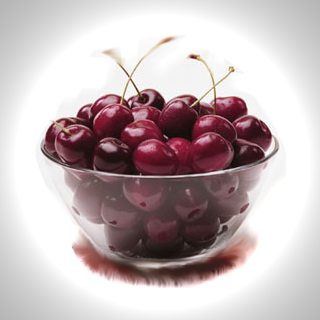
\includegraphics[width=0.33\textwidth]{figures/radiometric_before.png}}
  \subfigure[]{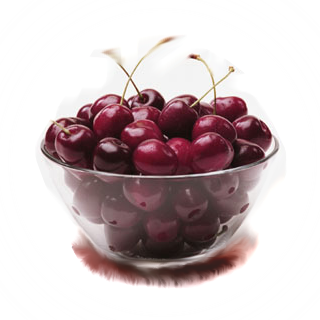
\includegraphics[width=0.33\textwidth]{figures/radiometric_after.png}}
 \end{center}
 \caption{
  Przykład zniekształceń radiometrycznych:
  (a) obraz zniekształcony;
  (b) obraz skorygowany.
 }
 \label{fig:radiometric}
\end{figure}

\subsubsection{Segmentacja}
Segmentacja obrazu to operacja polegająca na wydzieleniu z obrazu obszarów, które cechują się pożądanymi właściwościami (np. mają jednolitą barwę)~\cite{anal:przet:obr}.
Dostępne metody segmentacji to~\cite{roz:obr}:
\begin{itemize}
 \item metody punktowe:
  \begin{itemize}
   \item progowanie,
   \item klasteryzacyjne,
   \item metody krawędziowe,
  \end{itemize}
 \item metody obszarowe:
  \begin{itemize}
   \item rozrost obszarów,
   \item łączenie obszarów,
   \item podział obszarów,
   \item metoda podziału i łączenia,
   \item segmentacja wododziałowa,
  \end{itemize}
 \item metody hybrydowe (złożenie kilku metod).
\end{itemize}

Przykład poprawnej i niepoprawnej segmentacji obrazuje Rysunek~\ref{fig:segmentation}.

\begin{figure}[!ht]
 \begin{center}
  \subfigure[]{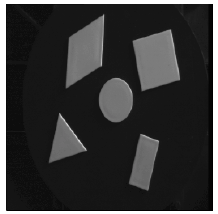
\includegraphics[width=0.25\textwidth]{figures/segmentation_before.png}}
  \subfigure[]{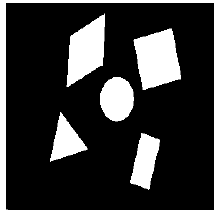
\includegraphics[width=0.25\textwidth]{figures/segmentation_proper.png}}
  \subfigure[]{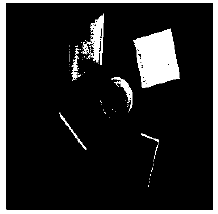
\includegraphics[width=0.25\textwidth]{figures/segmentation_improper.png}}
 \end{center}
 \caption{
  Przykład segmentacji:
  (a) obraz oryginalny;
  (b) obraz po poprawnej segmentacja;
  (c) obraz po niepoprawnej segmentacji.
  Źródło:~\cite{anal:przet:obr}.
 }
 \label{fig:segmentation}
\end{figure}

\subsubsection{Analiza i rozpoznanie}
Analiza i rozpoznanie obrazu polega na przeanalizowaniu wydzielonych segmentów obrazu i zidentyfikowaniu wśród nich tego zawierającego poszukiwany obiekt.
Klasyfikacja metod rozpoznawania obrazów wyszczególnia następujące grupy metod~\cite{roz:obr}:
\begin{itemize}
 \item metody minimalnoodległościowe,
 \item metody wzorców,
 \item metody aproksymacyjne,
 \item metody specjalne,
 \item metody probabilistyczne.
\end{itemize}

Przykład fotografii, na której rozpoznano ludzkie twarze, przestawia Rysunek~\ref{fig:face_detection}.

\begin{figure}[!ht]
 \begin{center}
  \scalebox{0.25}
  {
   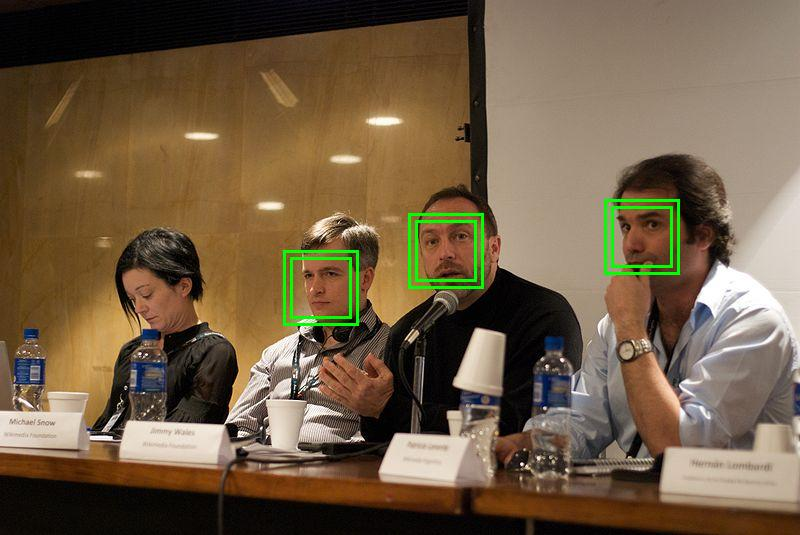
\includegraphics{figures/face_detection.jpg}
  }
 \end{center}
 \caption{
  Przykład rozpoznawania ludzkich twarzy na fotografii.
  Źródło: http://en.wikipedia.org/wiki/File:Face\_detection.jpg
 }
 \label{fig:face_detection}
\end{figure}


Aplikacja korzystać będzie z jednej lub kilku metod w celu podjęcia decyzji, czy (i gdzie) na obrazie z kamery urządzenia wyświetlić zapamiętany obraz.


Dodatkowo, wyświetlany obraz powinien być odpowiednio przetworzony, tak aby użytkownik miał wrażenie, że rzeczywiświe znajduje się on na wskazanej powierzchni.
Aby uzyskać pożądany efekt, obraz należy poddać odpowiednim przeksztaceniom geometrycznym.
Dostępne przekształcenia to między innymi~\cite{anal:przet:obr}:
\begin{itemize}
 \item przesunięcia,
 \item obroty,
 \item skalowanie,
 \item odbicia.
\end{itemize}

W tym przypadku wykorzystać należy obroty i skalowanie.

\subsubsection{Obracanie obrazu}
Wyświetlany obraz powinien zostać obrócony, tak aby zniwelować różnicę pomiędzy orientacją urządzenia w chwili umieszczenia, a jego orientacją w chwili wyświetlenia obrazu.


\subsubsection{Skalowane obrazu}
Skalowanie, czyli zmiana rozmiaru wyświetlanego obrazu~\cite{geo:tools}, powinno zostać wykonane, aby użytkownik mógł odnieść wrażenie zbliżania się do obrazu lub oddalania się od niego.

Współczynnik przeskalowania obrazu powinien być ustalony na podstawie porównania rozmiarów obiektów oryginalnego tła obrazu z ich rozmiarami na obrazie odczytanym przez kamerę urządzenia - współczynnik przeskalowania wyświetlanego obrazu powinien być równy stosunkowi tych rozmiarów.

Przykład obróconego i przeskalownego obrazu widoczny jest na Rysunku~\ref{fig:rotation_and_scale}.

\begin{figure}[!ht]
 \begin{center}
  \subfigure[]{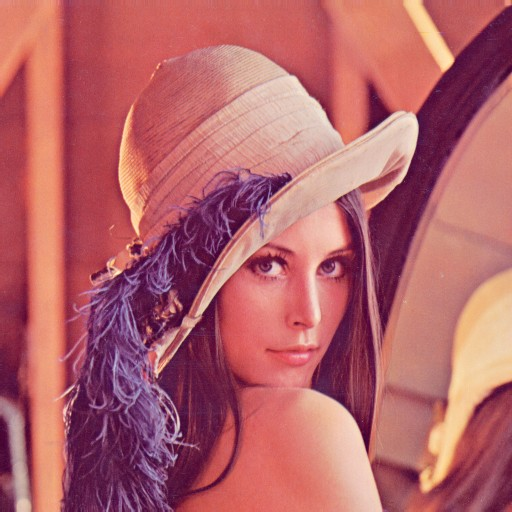
\includegraphics[width=0.33\textwidth]{figures/lena.jpg}}
  \subfigure[]{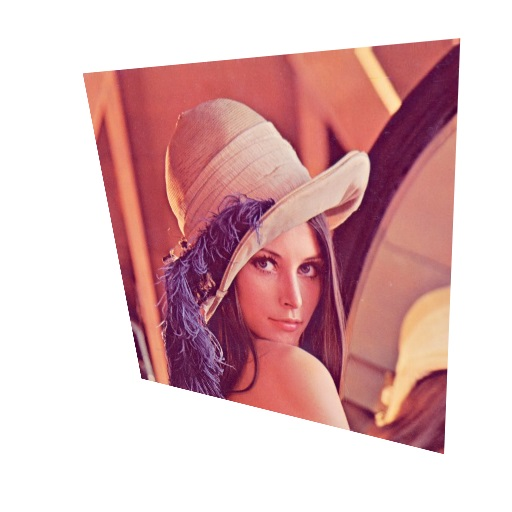
\includegraphics[width=0.33\textwidth]{figures/lena_rotated.jpg}}
 \end{center}
 \caption{
  Przykład obróconego i przeskalowanego obrazu:
  (a) obraz oryginalny;
  (b) obraz obrócony i przeskalowany.
 }
 \label{fig:rotation_and_scale}
\end{figure}

\subsection{Komunikacja klient-serwer}
Komunikacja pomiędzy klientem a serwerem może być zrealizowana przy użyciu różnych protokołów, takich jak:
\begin{itemize}
 \item UDP (User Datagram Procotol)~\cite{udp} - bezpołączeniowy (a więc zawodny) protokół komunikacyjny,
 \item TCP (Transmission Control Protocol)~\cite{tcp} - połączeniowy (niezawodny) protokół komunikacyjny,
 \item HTTP (Hypertext Transfer Protocol)~\cite{http1,http2}, jako \emph{web service}\footnote{https://pl.wikipedia.org/wiki/Usługa\_internetowa} wykorzystujący jeden z poniższych sposobów dostępu do danych:
  \begin{itemize}
   \item SOAP (Simple Object Access Protocol)~\cite{soap} - protokół wykorzystujący język XML, nie posiada ustandaryzowanego intefejsu (API),
   \item REST (Representational State Transfer)~\cite{rest} - wzorzec definiujący ustandaryzowany interfejs dostępu do danych, wspiera przesyłanie danych w języku XML lub formacie JSON,
   \item OData (Open Data Protocol)~\cite{odata} - protokół umożliwiający wygodne konstruowanie ustandaryzowanych zapytań o dane.
  \end{itemize}
\end{itemize}

Ponieważ komunikacja wewnątrz aplikacji odbywać się będzie według schematu żądanie-odpowiedź, strona serwerowa z powodzeniem może zostać zrealizowana jako \emph{web service}.
W chwili obecnej najbardziej popularne platformy umożliwiające tworzenie tego typu rozwiązań to .NET Framework (Microsoft)\footnote{Narzędzie Windows Communication Foundation (WCF)} i Java EE (Oracle)\footnote{Narzędzia: Java API for XML Web Services (JAX-WS) i  Java API for RESTful Web Services (JAX-RS)}.

\subsubsection{.NET}
Technologia WCF będąca częścią platformy .NET wspiera zarówno SOAP, jak i REST wraz z OData (jako rozszerzenie REST).

\subsubsection{Java EE}
Platforma Java EE posiada dwa narzędzia przeznaczone do budowy serwisów:
\begin{itemize}
 \item JAX-WS (Java API for XML Web Services) - wspiera serwisy wykorzystujące protokół SOAP,
 \item JAX-RS (Java API for RESTful Web Services) - służy to tworzenia serwisów opartych na REST (ang. \emph{RESTful}).
\end{itemize}

Nie posiada ona natywnego wsparcia dla protokołu OData - istnieją jednak implementacje przygotowane przez firmy trzecie: Google\footnote{OData4J (http://code.google.com/p/odata4j/)} i Apache\footnote{Apache Olingo (http://olingo.incubator.apache.org/documentation.html)}.

\subsection{Przechowywanie danych}
Aplikacja będzie przechowywać dane róznego rodzaju.
Będa to między innymi:
\begin{itemize}
 \item pliki obrazów umieszczanych przez użytkowników w wybranych miejscach,
 \item pliki zawierające tła tych obrazów,
 \item dane dotyczące właścicieli tych obrazów,
 \item dane dotyczące lokalizacji i orientacji telefonu w chwili umieszczenia obrazu w wybranym przez użytkownika miejscu.
\end{itemize}

O ile pliki graficzne mogą rezydować na dysku serwera bez konieczności utrzymywania ich w uporządkowanej strukturze, o tyle pozostałe dane powinny być zgrupowane i uporządkowane.
Najpopularniejszym sposobem przechowywania uporządkowanej struktury danych w tego typu aplikacjach jest wykorzystanie bazy danych.